\documentclass[11pt]{report}  %紙張設定
\usepackage{xeCJK}%中文字體模組
\setCJKmainfont{TW-Kai} %設定中文字體
%\setCJKmainfont{MoeStandardKai.ttf}
\usepackage[margin=2cm]{geometry}
\usepackage{graphicx}

%\第六章開始
\begin{document}
\begin{center} %文字置中
\Large\textbf{6.CHAPTER} %文字變大變粗
\end{center}
\Large\textbf{ODOOS ACOMPLISHMENTS REGARDING PLM AND 
MES}
\begin{center}
\Large\textbf{第六章}
\end{center}
\Large\textbf{ODOO 在產品生命週期管理 (PLM) 和製造執行系統 (MES) 方面的成就}\\

This chapter aims to summarize the strengths and weaknesses of the Odoo software 
focusing on the questions raised on section 4.2. It will also comment Odoo functionalities or 
lack thereof noticed throughout the simulation also taking the questions into account.\\
本章旨在概述Odoo軟件的優點和缺點,重點關注第4.2節提出的問題。同時也將評論在模擬過程中注意到的Odoo功能或缺失,並考慮這些問題。\\

\Large\textbf{6.1.How does the software deals with items?}
\Large\textbf{6.1 軟體如何處理物品?}\\

Overall, the Odoo software presents the user with a wide variety of digital items that can 
be used to represent several aspects of manufacturing as well as other aspects of business. 
This is mainly due to the way the Odoo ERP functionality uses items to track the pull and 
push actions throughout its use, that is also how automation is achieved in the software.\\
整體而言,Odoo 軟件向用戶提供了各種數字項目,可以用來代表製造業的各個方面以及業務的其他方面。這主要是由於 Odoo ERP 功能使用項目來跟蹤其使用過程中的拉動和推動動作,這也是軟件中實現自動化的方式。\\

\Large\textbf{6.1.1. Are all aspects of the product lifecycle represented?}\\
\Large\textbf{6.1.1. 產品生命週期的所有方面都有所代表嗎?}\\

One of the disadvantages of being derived from a ERP system is that it focus on the 
primary scope of ERP (Figure 2) ,that is, production and sales. The Items in Odoo reflect 
that. For instance, the development part of the life cycle during the simulation, although the 
representation was possible it certainly felt like a stretch of functionalities made for the 
production phase rather than development is self (Figure 70). When developing prototypes 
for instance many of the steps like creating an ECO just to carry files in the beginning and
going through many steps every time an adjustment in the prototype was made felt too
bureaucratic or too much of a workaround.\\
由ERP系統衍生出來的一個缺點是它專注於ERP的主要範圍(見圖2),即生產和銷售。Odoo中的項目反映了這一點。例如,在模擬期間,生命週期的開發部分,雖然表示是可能的,但確實感覺像是針對生產階段而非開發本身所進行的功能延伸(見圖70)。例如,在開發原型時,許多步驟,如一開始只是創建一個 ECO 來攜帶文件,以及每次調整原型時都要進行許多步驟,感覺太過於官僚主義或是太過於繞彎。\\

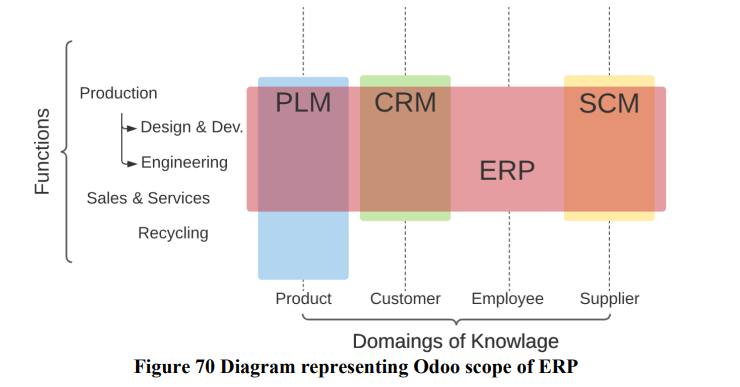
\includegraphics[]{6-1.png}\\%加入6-1圖片%%%%%%%%%%%%%%%%

\Large\textbf{6.1.2. How well are each of those items represented?}\\
\Large\textbf{6.1.2. 這些項目的代表程度如何?}\\

Representation levels of the items vary depending on how the item is used. A good 
example of that is the material focus of product items. In the sense that everything is 
considered a product with very little distinction between prototypes or raw materials. The 
representation of product items or BOM items is very high with a lot of metadata and useful 
connections to other items. However, even within the manufacturing application there are 
some items that lack attention. Operations for instance are items that could benefit greatly 
from more upload capabilities like 3D printing or CNC files. As automation is becoming 
more widespread in production it is no longer enough to have only PDF or slide instructions.
Additionally, other items do not have the ability of holding files not even with the use of 
ECOs\\
項目的代表程度取決於該項目的使用方式。一個很好的例子是產品項目的材料焦點。從這個意義上說,一切都被認為是產品,幾乎沒有原型或原材料之間的明確區別。產品項目或BOM項目的表示非常高,具有許多元數據和與其他項目的有用連接。然而,即使在製造應用程序中,也有一些項目缺乏關注。例如,操作是一種可以從更多上傳功能中受益的項目,如3D打印或CNC文件。隨著自動化在生產中變得越來越普遍,僅僅擁有PDF或幻燈片說明已不再足夠。此外,其他項目甚至沒有保留文件的能力,即使使用了ECO也不行。\\

\Large\textbf{6.2.How easy it is to create a brand-new product?}\\
\Large\textbf{6.2 創建全新產品有多容易?}\\

Product creation is one of the most straightforward procedures in Odoo, it really comes 
down to using either the Inventory application or the Manufacturing application to create a 
new Product and then fill in its metadata.\\
在Odoo中,產品創建是最直接的程序之一,實際上只需要使用庫存應用程序或製造應用程序來創建一個新產品,然後填入其元數據即可。\\

\Large\textbf{6.2.1. How is the product depicted?}
\Large\textbf{6.2.1. 產品如何描述?}\\

The product depiction is clear and concise, the product item allows for an image to be 
uploaded to the item and used as an icon. The ERP nature of the product items in Odoo means 
that the metadata is reasonably bias toward information that is used to manage storage and 
inventory (Weight, Volume, Quantity etc.) but the item also allows for written description 
as well as providing links to the BOMs and ECOs related to the product.\\
產品描述清晰簡潔,產品項目允許上傳圖像並用作圖標。Odoo中產品項目的ERP性質意味著元數據相對偏向於用於管理存儲和庫存的信息(重量、體積、數量等),但該項目還允許撰寫描述,並提供與產品相關的BOM和ECO的鏈接。\\

\Large\textbf{6.2.2. How does the product integrate and reference relevant files?}\\
\Large\textbf{6.2.2. 產品如何整合和參考相關文件?}\\

There is surely a reasonable attempt in allowing the most valuable items (Product and 
BOMs) to be able to manage and reference relevant files. However, Odoo does not implement 
much more than the bare minimum as far as file management goes. The most it can do is 
allow for files to be uploaded and download manually. This means that whenever someone 
makes a change in a file it needs to be manually uploaded in ECO. Integration with most files 
is inexistent except for operation items because the instruction files can be opened and 
interacted within Odoo during the production.\\
Odoo 確實試圖允許最有價值的項目(產品和 BOM)能夠管理和參考相關文件。然而,在文件管理方面,Odoo 的實現不多於基本的最低要求。它最多只能允許手動上傳和下載文件。這意味著每當有人對文件進行更改時,都需要手動在 ECO 中上傳。與大多數文件的集成幾乎不存在,除了操作項目,因為在生產過程中可以在 Odoo 中打開和交互指示文件。\\

\Large\textbf{6.2.3. Does changing one affects the other?}\\
\Large\textbf{6.2.3.更改其中一個是否會影響另一個?}\\

It does not, files are mostly dealt by Odoo as paperwork for later reference. Anything 
added file wise that could entail a change in the product or BOM metadata will require
someone to be aware of the change and update the information manually.\\
不會,文件在大多數情況下由Odoo作為以後參考的文件處理。任何增加的文件,如果可能導致產品或BOM元數據的變更,都需要有人注意到這一變更並手動更新信息。\\

\Large\textbf{6.3.How easy it is to create a brand-new production process?}\\
\Large\textbf{6.3 創建全新的生產流程有多容易?}\\

As mentioned before the item the best represents the process is the bill of materials. This 
item class requires an existing product to be associated with, other that the BOM is no harder 
to create than a product item.\\
如前所述,最能代表流程的項目是物料清單。這個項目類別需要與現有產品相關聯,除此之外,創建 BOM 的難度與創建產品項目一樣。\\

\Large\textbf{6.3.1. How the process is depicted?}\\
\Large\textbf{6.3.1. 流程是如何描述的?}\\

The process is depicted in the BOM as a list of components (other product items) and 
operations that are carried out in as specific order to produce a number of end products. This 
representation seems to sit well with the production procedure. Metadata is kept to a 
minimum but there is still the capability to offer a text description.\\
流程在 BOM 中被描述為一個組件列表(其他產品項目)和按特定順序進行的操作,以生產一定數量的最終產品。這種表示方式似乎很適合生產程序。元數據被保持在最低限度,但仍有提供文本描述的能力。\\

\Large\textbf{6.3.2. How does the process integrate and reference the product it produces?}\\
\Large\textbf{6.3.2. 流程如何整合和參考其生產的產品?}\\

The integration between the BOM and the product items is by far the most well done in 
Odoo. Changes made in the BOM affect production and are directly linked to the product. 
Whenever metadata changes are possible and said aspect is represented in the product item 
as well the change of one is inherited by the other.\\
在Odoo中,BOM和產品項目之間的整合是最成功的。在BOM中進行的更改會影響生產並直接與產品相關聯。每當元數據的更改是可能的,並且該方面在產品項目中也被表示時,其中一個的更改將被另一個繼承。\\

\Large\textbf{6.3.3. Does changing one affects the other?}\\
\Large\textbf{6.3.3.更改其中一個是否會影響另一個?}\\

As far as inventory and manufacturing is concerned integration is and referencing is well 
implemented. Production results flawlessly in the resulting changes in inventory and the 
navigation path of the GUI is very well optimized. It does not take more than 3 or 4 clicks 
to get from one product to another or to navigate to other relevant items.\\
就庫存和製造而言,整合和參考都得到了很好的實現。生產過程中庫存的變化無瑕地反映出來,GUI 的導航路徑非常優化。從一個產品轉到另一個產品,或者導航到其他相關項目,不需要超過3或4次點擊。\\

\Large\textbf{6.4.How easy is to improve an existing product/ production process?}\\
\Large\textbf{6.4 改善現有產品/生產流程有多容易?}\\

 As mentioned previously, all improvements in Odoo are performed using engineering 
change orders. These are applied to product items or bill of materials. Creating ECOs is quite 
easy and organized, the ECO is an item on itself that symbolizes a signal given to create 
change, once effective, it symbolizes an increment on the product or process.\\
如前所述,Odoo 中的所有改進都是使用工程變更訂單執行的。這些應用於產品項目或物料清單。創建ECO相當容易和有組織,ECO本身就是一個項目,象徵著創建變更的信號,一旦生效,它象徵著產品或流程的增量。\\

\Large\textbf{6.4.1. How easy it is to update its metadata?}\\
\Large\textbf{6.4.1 更新元數據有多容易?}\\

It is easy to update any metadata regarding any item in Odoo; however, it is wise to point 
out that since the ECOs are separate items that are just point by products or BOMs many of the changes are not automatic and require manual intervention. I.e. an ECO will not change the text description of the product for instance. If the new update were to require a change on that description it would require a manual intervention from the user in the product item. 
Doing that is easy, but it is an extra task that will not be tracked by the ECO.\\
在Odoo中更新任何項目的任何元數據都很容易;然而,明智的是要指出,由於ECO是獨立的項目,只是指向副產品或BOM,許多更改不是自動的,需要手動干預。例如,ECO不會更改產品的文字描述。例如,如果新更新需要更改該描述,則需要用戶在產品項目中進行手動干預。這樣做很容易,但這是一項額外的任務,不會被ECO跟踪。\\

\Large\textbf{6.4.2. How easy it is to determine the effects of the change?}\\
\Large\textbf{6.4.2 確定更改的影響有多容易?}\\
    
Odoo feedback of information is mainly done in a manufacturing order basis. The 
information available is clear and ECOs do not affect MOs that are already under way so the 
effects of an applied ECO would not be hard to notice. However, it is good to point out that 
in the way the performance information is displayed there is no indication of the product 
revision or the ECO applied. This means that the user would need to first figure when the 
ECO was applied, then navigate to the equivalent MO in the data to draw its conclusions. 
Although not a problem for recent changes this does becomes problematic if someone want 
to analyze effects of old changes.\\
在Odoo中,信息反饋主要是以製造訂單為基礎的。可用信息清晰明確,ECO不會影響已經進行中的MO,因此應用的ECO的影響不難察覺。然而,值得指出的是,在顯示性能信息的方式中,沒有顯示產品修訂版或應用的ECO的指示。這意味著用戶首先需要弄清楚何時應用了ECO,然後導航到數據中的相應MO,才能得出結論。儘管對於最近的更改沒有問題,但如果有人想分析舊更改的影響,這就變得棘手了。\\

\Large\textbf{6.4.3. How does the software deals with different product revisions?}\\
\Large\textbf{6.4.3. 軟體如何處理不同的產品修訂?}\\

Version control is something well covered by the 1 to N relation between product/BOM 
and linked ECOs. Every product will have a tab containing all the ECOs applied to it in 
chronological order effectively working as a timeline representing the item evolution. \\
版本控制在產品/BOM和相關的ECO之間的1對N關係中得到了很好的覆蓋。每個產品將具有包含應用到該產品的所有ECO的選項卡,按時間順序排列,有效地充當代表項目演變的時間軸。\\

\Large\textbf{6.5.How easy is to find data related to product or process?}\\
\Large\textbf{6.5 查找與產品或流程相關的數據有多容易?}\\

Most of the data related to performance regarding production is concentrated under the reporting tab as mentioned in the previous chapter (Figure 71).\\
大部分關於生產性能的數據都集中在報告選項卡下,如前一章節所述(見圖71)。\\
\begin{center}
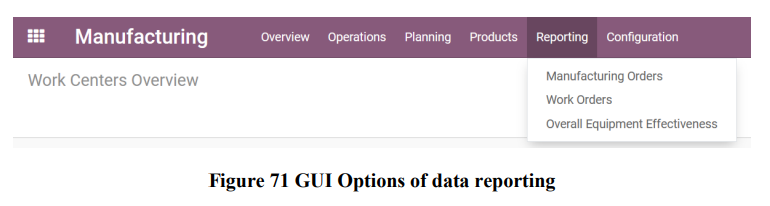
\includegraphics[]{6-2.png} %插入6-2圖片並保持置中%%%%%%%%%
\end{center}
This means that as far as performance is concerned it is quite easy to find the data. The previous chapter will show examples of possible information that are available within those tabs. In addition to using this path the UI of the product item also has a tab that point to the monthly comparison of production volume regarding the product (Figure 72). Which would be more impressive if there was more than one month in the trial version of Odoo.\\
這意味著就性能而言,查找數據相當容易。前一章節將展示在這些選項卡中可用的可能信息示例。
除了使用這個途徑外,產品項目的 UI 也有一個標籤,指向有關該產品的月度生產量比較(見圖 72)。如果 Odoo 的試用版本中有多個月份的話,這將更為印象深刻。\\
\begin{center}
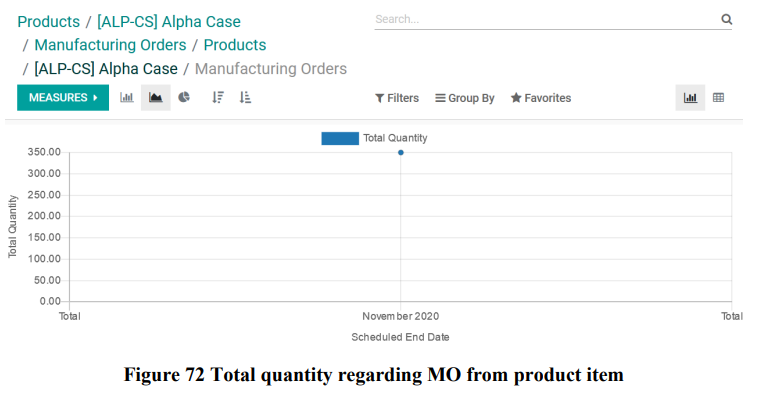
\includegraphics[]{6-3.png}%插入6-3圖片並保持置中%%%%%%%%%
\end{center}
\Large\textbf{6.5.1. How easy is find production numbers?}\\
\Large\textbf{6.5.1 找到生產數字有多容易?}\\

In addition to the previously mentioned ways, Odoo also makes available a unit forecast graph that records the ins and outs of the inventory. This is particularly useful to estimate sales and balance storage with demand (Figure 73). This feature is not mentioned to much in this work because supply and demand is not so much a MES functionality, but it is to useful 
to have an overview of the production.\\
除了之前提到的途徑外,Odoo還提供了一個單位預測圖表,記錄庫存的進出情況。這對於估計銷售並平衡庫存與需求特別有用(見圖 73)。雖然這個功能在本文中沒有被提及太多,因為供需不是 MES 功能的主要內容,但對於獲得生產概覽是非常有用的。\\
\begin{center}
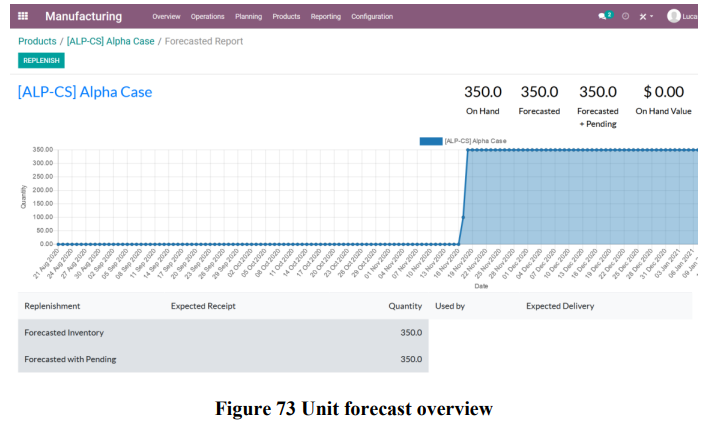
\includegraphics[]{6-4.png}%插入6-4圖片並保持置中%%%%%%%%%
\end{center}
\Large\textbf{6.5.2. How does Odoo generate performance data?}\\
\Large\textbf{6.5.2. Odoo 如何生成性能數據?}\\

The astute reader will notice that all the data mentioned so far is derived from the time to completion of the operations been carried out, the related amount to the MO and the workcenter utilized. Even so it is impressive how much information can be drawn especially considering that it is all generated automatically.\\
機警的讀者會注意到到目前為止提到的所有數據都是從操作完成所需的時間、相關的 MO 量以及使用的工作中心派生出來的。儘管如此,特別考慮到所有這些信息都是自動生成的,可以提取出多少信息仍然令人印象深刻。\\

\Large\textbf{6.5.3. How does the software present performance change as a result of a upgrade?}\\
\Large\textbf{6.5.3. 軟體如何呈現升級導致的性能變化?}\\

In order to identify the change, the user must identify the MOs following the change and see the difference based on that. Ideally it would be nice if the graphical information showed the revision of the product, but this is not present as of Odoo V13.\\
為了識別變化,用戶必須確定變化後的 MO,並根據此進行比較。理想情況下,如果圖形信息顯示了產品的修訂,那將是很好的,但截至 Odoo V13 目前尚未實現。
\end{document}


